\section{Structured results}\label{results}

\[
\begin{aligned}a&=1\\b&=-2\end{aligned}
\]

\[
\begin{bmatrix}0&-1\\2&3\end{bmatrix}
\]

\begin{figure}
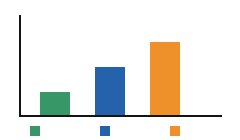
\includegraphics{assets/figure-en.png}
\caption{Figure 1 — Three regions and laboratory axes.}\label{fig1}
\end{figure}

See the figure and the source while keeping references explicit. \ref{fig1} \href{https://example.invalid/study?series=0012\&mode=a_b#note}{source} \cite{bib1}

\begin{thebibliography}{1}
\bibitem{bib1}Synthetic Researcher. Source notebook, 2026.
\end{thebibliography}

